\documentclass[8pt]{beamer}
\usepackage[T1]{fontenc} 
\usepackage[francais]{babel}
\usepackage{tikz}
\usetikzlibrary{arrows,shapes}
\usepackage{pslatex}
\usepackage{textcomp}
\usepackage[utf8]{inputenc}  
\usepackage{wrapfig}
\usepackage{graphicx}
\usepackage[section]{placeins}
\usepackage{lscape}
\usepackage{float} 
\usepackage{amssymb}
\usepackage{wasysym}
\usepackage{pgf}
\usepackage{alltt}
\usepackage{eso-pic}
\usepackage{url}
\usepackage{tikz}
\usepackage{listings}
\usepackage{color}
\definecolor{mymauve}{rgb}{0.58,0,0.82}

\lstset{language=C++,
basicstyle=\footnotesize,
keywordstyle=\color{red}\bfseries,
breaklines=true,
commentstyle=\color{blue},
stringstyle=\color{mymauve},
literate={ô}{{\^o}}1 {é}{{\'e}}1 {à}{{\`a}}1 {è}{{\`e}}1 {î}{{\^{\i}}}1 {ê}{{\^e}}1 {ç}{{\c c}}1,
morekeywords={string,fstream,ofstream,ifstream}
}
\usepackage{hyperref}

%\hypersetup{urlcolor=blue}

\usetheme{CambridgeUS}


\title[DQM4HEP - v03-02-00]{Data Quality Monitoring for High Energy Physics (DQM4HEP) \\ Module interfaces}
\institute[UCBL - IPNL - UGent]{Université Claude Bernard Lyon 1 - Institut de Physique Nucléaire de Lyon / Ghent University}
\author[Eté - Pingault - Mirabito]{{\bf \large R. \'Eté, A. Pingault, L. Mirabito}}
\date{\today}

\DeclareUnicodeCharacter{00A0}{ }

\setbeamertemplate{itemize items}[ball]
\definecolor{MyGreen}{rgb}{0.1,0.5,0.1}
\setbeamercolor{structure}{fg=red!70!black}
\setbeamercolor{block title}{bg=red!70!black,fg=black}
\addtobeamertemplate{block begin}{\pgfsetfillopacity{0.5}}{\pgfsetfillopacity{1}}

\begin{document}


  %%%%%%%%%%%%%% Page de présentation %%%%%%%%%%%%%%
  \begin{frame}

    \titlepage
    \begin{center} 
      
\includegraphics[width=0.5\textwidth]{logo/logo-ucbl-ipnl.jpg} ~~~~~~~~~~~
      
\includegraphics[width=0.2\textwidth]{logo/Ghent_University_logo.png}
    \end{center}
  \end{frame}
  
  %% Architecture %%
  \begin{frame}
    \frametitle{Global workflow}
    
    \begin{center}
      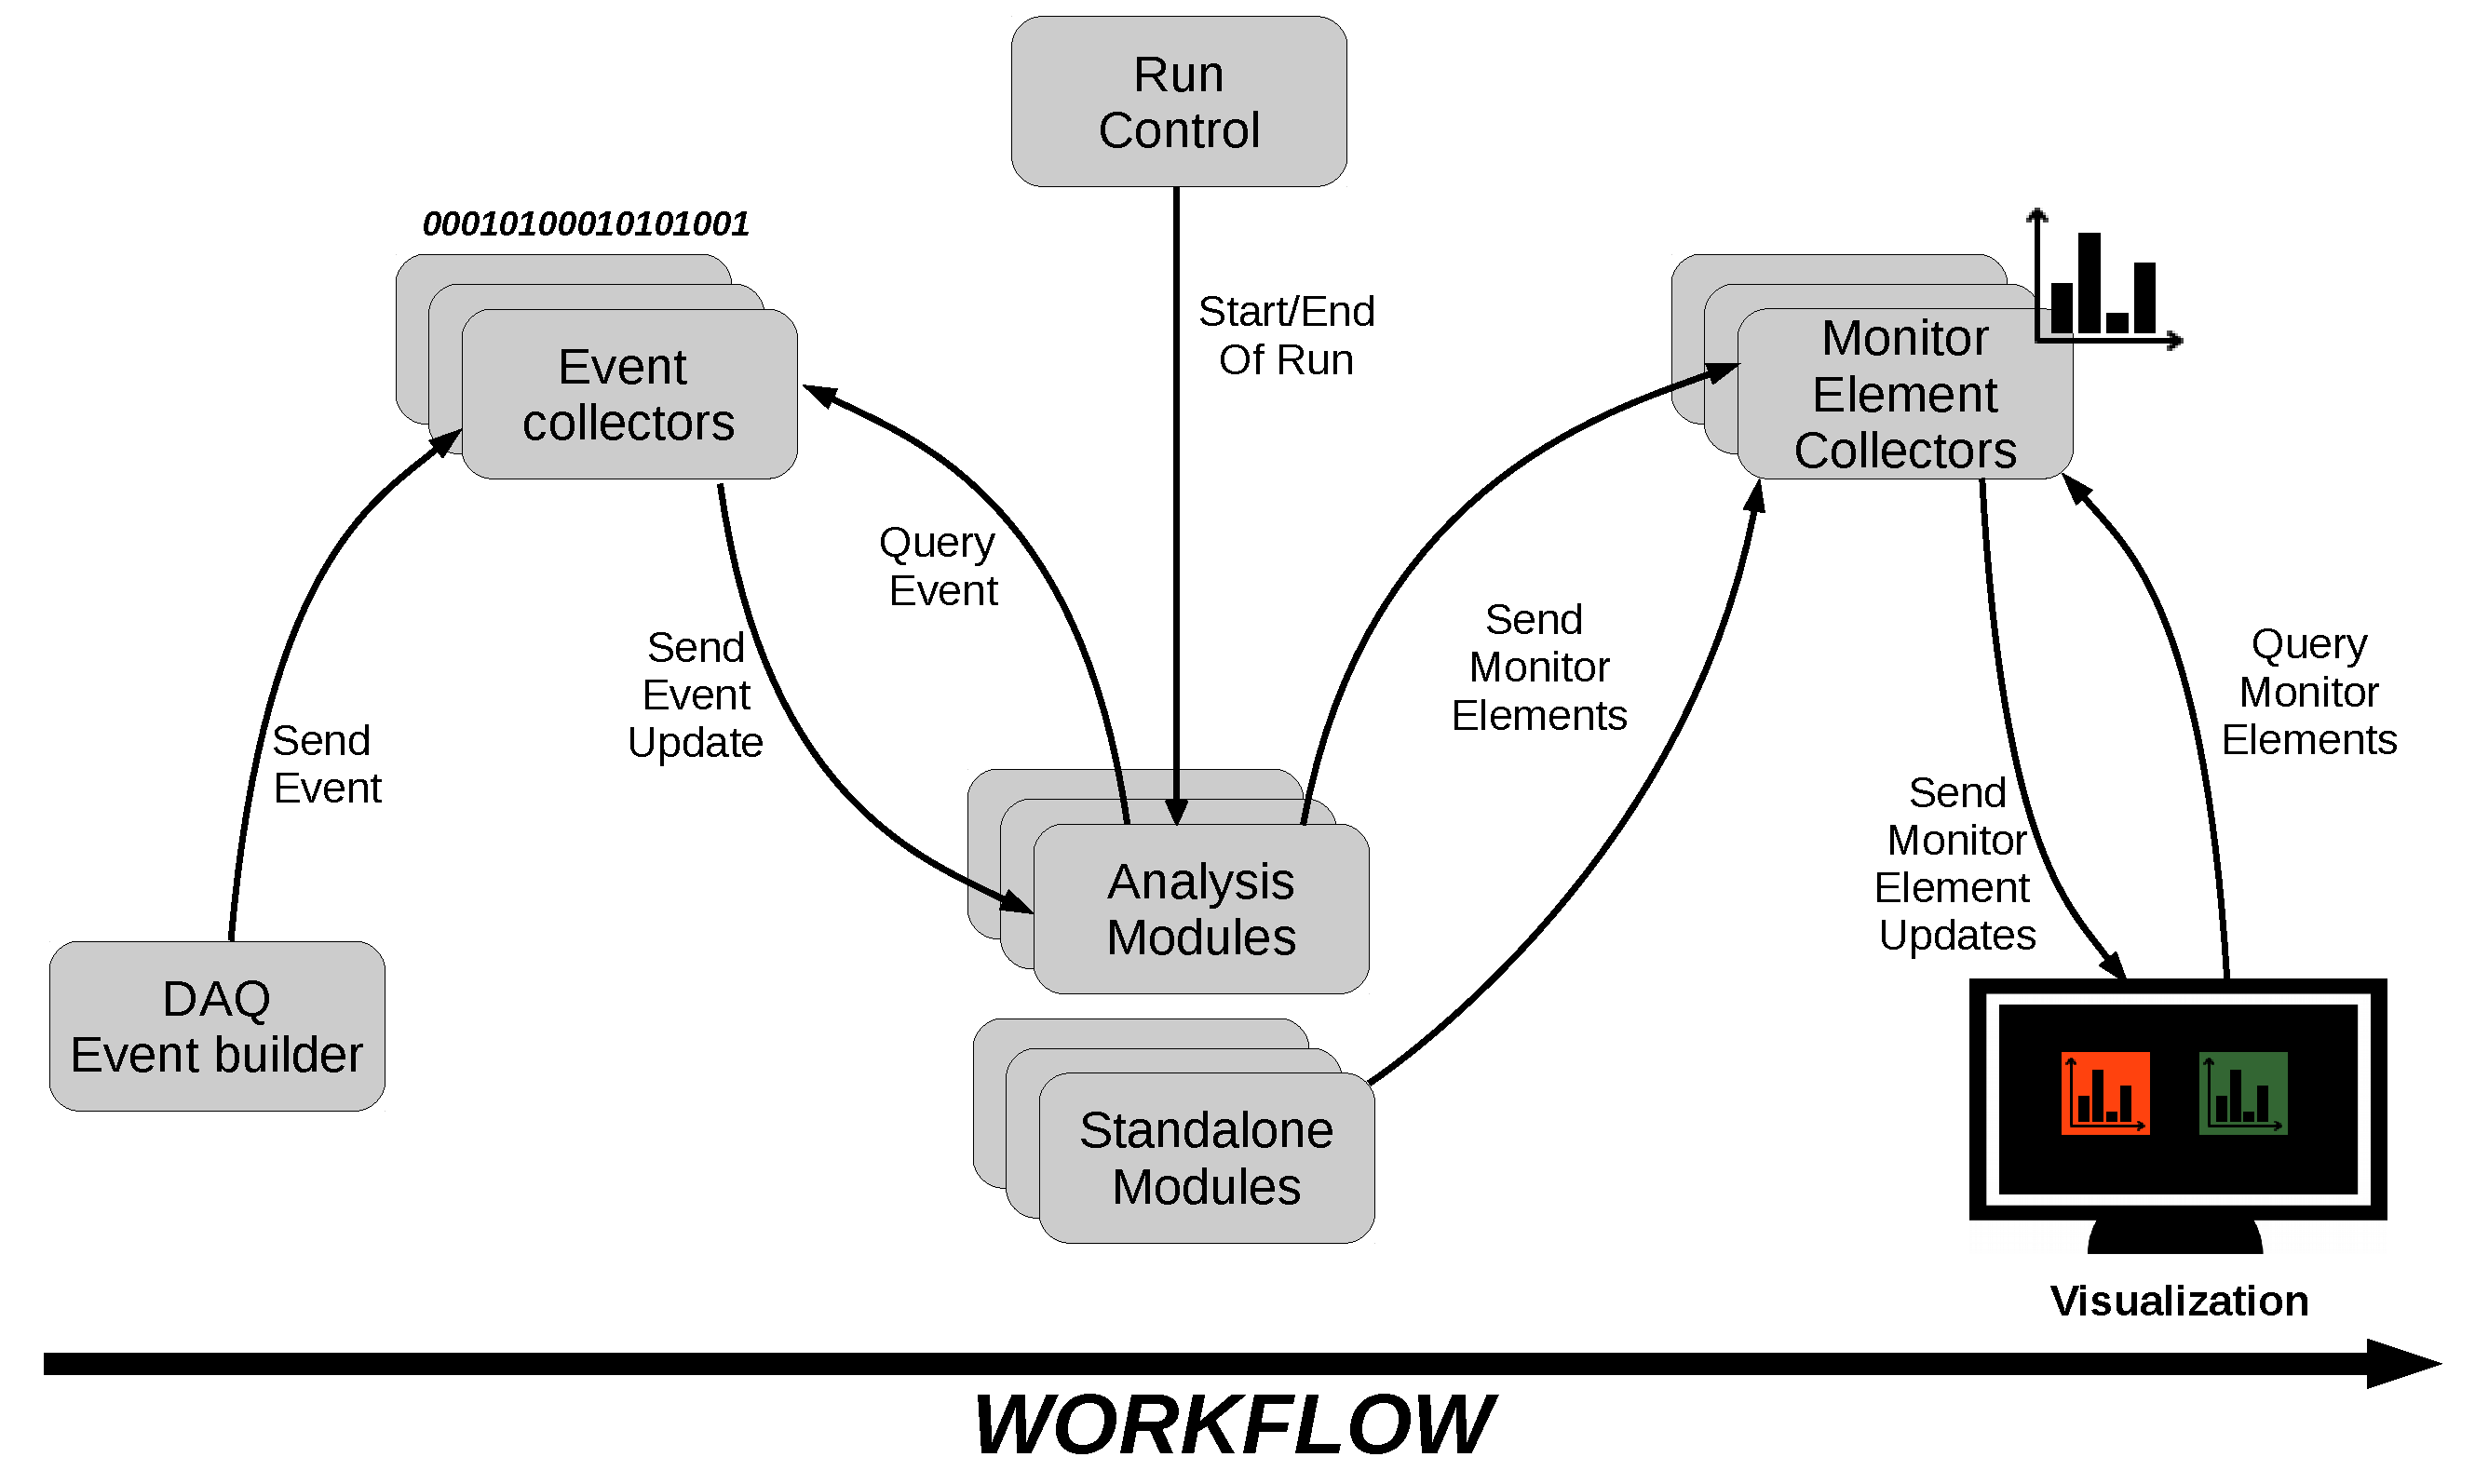
\includegraphics[width=\textwidth]{figs/DQM4HEP_workflow.pdf}        
    \end{center}
  
  \end{frame}
  
  
  %% MODULE APPLICATION %%
  \begin{frame}[containsverbatim]
    \frametitle{Module applications - analysis module}
    
    \begin{minipage}{0.78\textwidth}
      \begin{block}{Purpose}
        \begin{itemize}
          \item Receive events from a collector server and process them
          \item Produce monitor elements (histograms, scalars, generic TObject)
          \item Follow the run control signals (SOR, EOR)
        \end{itemize}
      \end{block}
              
      \begin{itemize}
        \item \textbf{Init} : Initialize the application : load dlls, declare services, etc ... Wait for a SOR
        \item \textbf{Start of run} : start cycles loop, open archive
        \item \textbf{Start of cycle} : start a cycle of '\textit{process event}'
        \item \textbf{Process event} : Process incoming event, fill monitor elements, etc ...
        \item \textbf{End of cycle} : send subscribed monitor elements, update archive (opt). 
        \item \textbf{End of run} : Wait for SOR, close archive (opt).
        \item \textbf{End} : Clean and exit module.
      \end{itemize}
      To implement online DQM analysis, user must implement the \verb|DQMAnalysisModule| interface. A shared library must be build and loaded in the application using the plugin system (see next slides). \\
      ~ \\
      Use \verb|dqm4hep_start_analysis_module| to start an analysis module.
        
    \end{minipage}
    \begin{minipage}{0.2\textwidth}
      \begin{flushright}
        \begin{tikzpicture}[scale=0.8]
        \node[draw] (I) at (0,-1) {Init};
        \node[draw] (SR) at (0,-2) {Start of run};
        \node[draw] (SC) at (0,-3) {Start of cycle};
        \node[draw] (PE) at (0,-4) {Process event};
        \node[draw] (EC) at (0,-5) {End of cycle};
        \node[draw] (ER) at (0,-6) {End of run};
        \node[draw] (E) at (0,-7) {End};
        \tikzset{fleche/.style={->,>=latex,thick}}
        \draw[fleche] (0,0) node {$\bullet$} -- (I);
        \draw[fleche] (I) -- (SR);
        \draw[fleche] (SR) -- (SC);
        \draw[fleche] (SC) -- (PE);
        \draw[fleche] (PE) -- (EC);
        \draw[fleche] (EC) -- (ER);
        \draw[fleche] (ER) -- (E);
        \draw[fleche] (E) -- (0,-8) node {$\bullet$};
        \draw[fleche] (0,-4.5) -- (1.3,-4.5) -- (1.3,-3.5) -- (0,-3.5);
        \draw[fleche] (0,-5.5) -- (1.4,-5.5) -- (1.4,-2.5) -- (0,-2.5);
        \draw[fleche] (0,-6.5) -- (1.5,-6.5) -- (1.5,-1.5) -- (0,-1.5);
        \end{tikzpicture}\\
        Analysis module~~~~\\ application flow~~~~~      
      \end{flushright}
    \end{minipage}
    
  \end{frame}
  
  \begin{frame}
    \frametitle{Module API}
      \begin{center}
       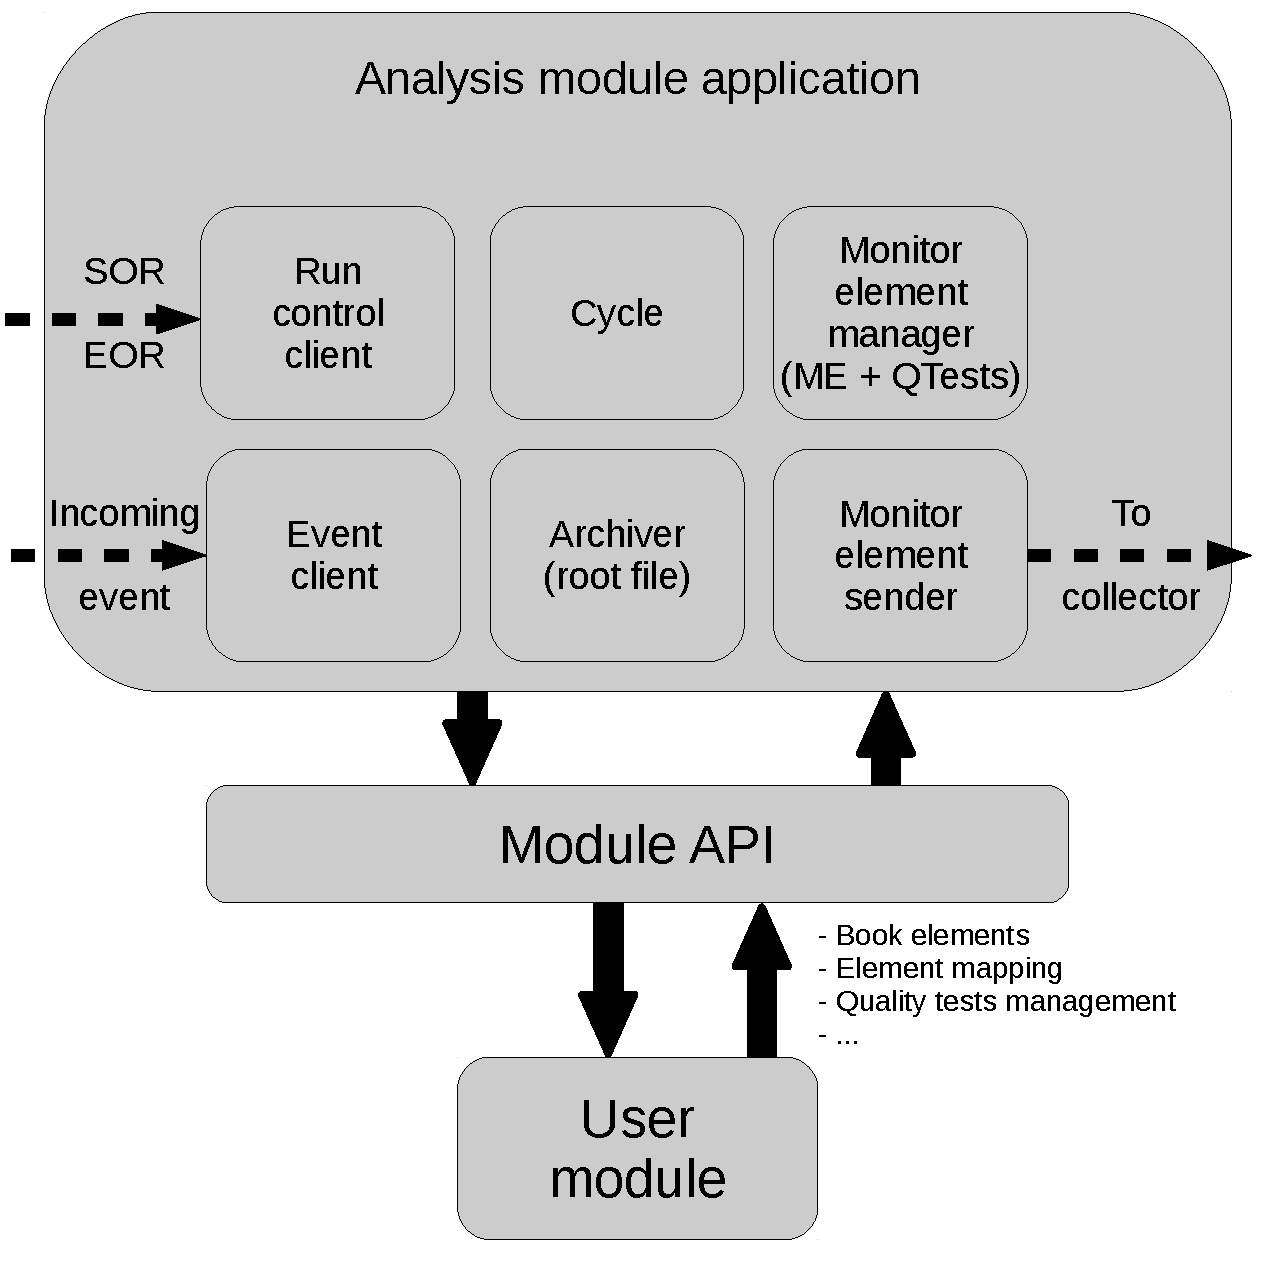
\includegraphics[width=0.6\textwidth]{figs/analysis_module_api.pdf}        
      \end{center}
  \end{frame}
  
  
  \begin{frame}[containsverbatim]
    \frametitle{Module applications - standalone module}

    \begin{minipage}{0.78\textwidth}
      \begin{block}{Purpose}
        \begin{itemize}
          \item No event reception
          \item No run signals
          \item Produce monitor elements (histograms, scalars, generic TObject)
        \end{itemize}
      \end{block}
      
      \begin{itemize}
        \item \textbf{Init} : Load dlls, init the module.
        \item \textbf{Start of cycle} : start a timer cycle of n seconds
        \item \textbf{Process} : call back function.
        \item \textbf{End of cycle} : collect monitor elements and send
        \item \textbf{End} : The application has received a signal to exit and the process ends.
      \end{itemize}
      To implement online standalone analysis, user must implement the \verb|DQMStandaloneModule| interface. A shared library must be build and loaded in the application using the plugin system (see next slides). \\
      ~ \\
      \textcolor{red}{Designed for \textit{slow control - like} data processing}. \\
      ~ \\
      Use \verb|dqm4hep_start_standalone_module| to start a standalone module.
    \end{minipage}
    \begin{minipage}{0.2\textwidth}
      \begin{flushright}
        \begin{tikzpicture}[scale=0.8]
        \node[draw] (I) at (0,-1) {Init};
        \node[draw] (SC) at (0,-2) {Start of cycle};
        \node[draw] (PE) at (0,-3) {Process};
        \node[draw] (EC) at (0,-4) {End of cycle};
        \node[draw] (E) at (0,-5) {End};
        \tikzset{fleche/.style={->,>=latex,thick}}
        \draw[fleche] (0,0) node {$\bullet$} -- (I);
        \draw[fleche] (I) -- (SC);
        \draw[fleche] (SC) -- (PE);
        \draw[fleche] (PE) -- (EC);
        \draw[fleche] (EC) -- (E);
        \draw[fleche] (E) -- (0,-6) node {$\bullet$};
        \draw[fleche] (0,-3.5) -- (1.3,-3.5) -- (1.3,-2.5) -- (0,-2.5);
        \draw[fleche] (0,-4.5) -- (1.4,-4.5) -- (1.4,-1.5) -- (0,-1.5);
        \end{tikzpicture} \\
        Standalone module~~~~\\ application flow~~~~~~~
      \end{flushright}
    \end{minipage}
    
  \end{frame}
  
  \begin{frame}
    \frametitle{Module API}

      \begin{center}
        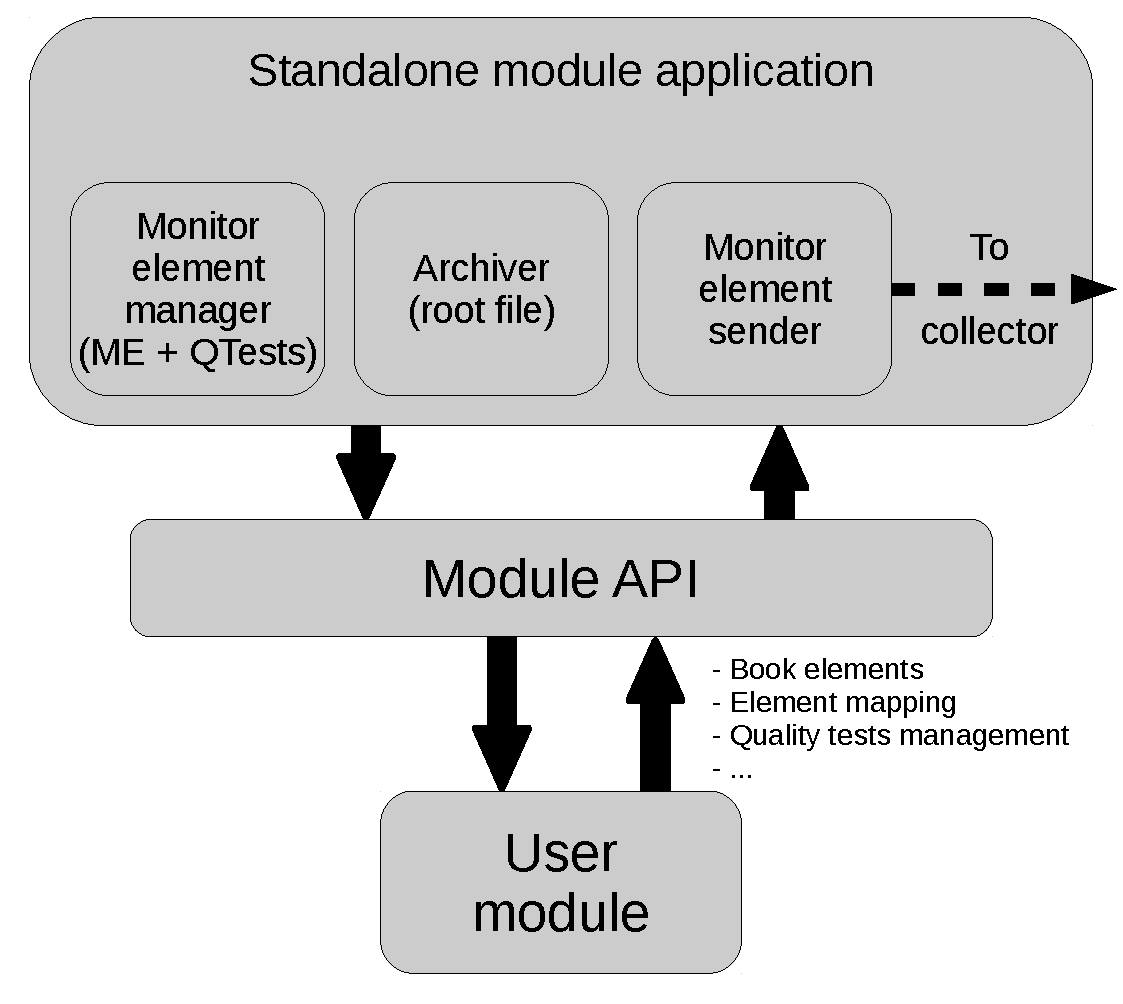
\includegraphics[width=0.6\textwidth]{figs/stand_module_api.pdf}        
      \end{center}
  \end{frame}
    
    %% MODULE API %%
    \begin{frame}[containsverbatim]
      \frametitle{Module API}
      
      Data processing performed in \textbf{modules} (standalone or analysis). \\
      Modules \textbf{book} monitor elements, \textbf{fill} them and \textbf{publish} them to a single collector. \\
      ~ \\
      A monitor element is a wrapper around a ROOT TObject with some additional attributes : \\
      $\rightarrow$ Type, name, path (i.e "/Efficiency/Layer2/"), collector name, quality flag, reset policy, title, description, run number, quality test results. \\
      ~ \\
      The \verb|DQMModuleApi| class provide a static interface to perform operations within the application :
      \begin{itemize}
        \item Monitor elements management (book, delete, reset, from xml)
        \item Directory structure management (mkdir, cd, ls, rmdir, pwd)
        \item Quality test management (register, add, remove, run, from xml)
      \end{itemize}
      ~ \\
      Quality tests can be run on a particular monitor element to test the quality of the processed data (chi2, Kolmogorov, user defined). \\ 
      ~ \\
      Note that \textbf{QTest results are sent to the collector together with the monitor element} ! 
    \end{frame}
    
    \begin{frame}[containsverbatim]
      \frametitle{Example modules}
      
      An LCIO example module can be found on the github page of DQMCore package \href{https://github.com/DQM4HEP/DQMCore}{\tt https://github.com/DQM4HEP/DQMCore} : \\
      ~ \\
      CaloHitModule (lcio, analysis) :
      \begin{itemize}
        \item source/examples/module/lcio/CaloHitModule.h
        \item source/examples/module/lcio/CaloHitModule.cc
        \item conf/lcioCaloHit.xml
        \item \verb|dqm4hep_start_analysis_module| executable
      \end{itemize}
    \end{frame}
  
\end{document}
